近年来,人工智能(AI)和机器学习(ML)越来越受到人们的青睐。从简单的送餐网站,到复杂的工业机器人,人工智能已成为软件和硬件的主要功能之一。虽然在大多数情况下,这些术语都是为了让产品看起来更严肃,但一些公司正在深入研究并将人工智能融入自己的系统。 \par
在进一步讨论之前,请考虑以下事实:本章从C++开发者的角度对ML进行了介绍。要了解更全面的文献,请参阅本章末尾的书单。在这一章中,我们将介绍AI和ML的概念。虽然我们更倾向于有数学背景,但在这一章中我们几乎不使用任何数学。如果你正计划扩大你的技能集和潜入ML,必须首先考虑学习数学。 \par
除了介绍概念,本章还提供了ML任务的例子。我们将实现它们,并给你一个基本的想法,你应该如何研究和前进,以解决更复杂的任务。 \par

本章中,我们将了解以下内容: \par

\begin{itemize}
	\item 介绍AI和ML
	\item ML的分类和应用
	\item 设计用于计算的C++类
	\item 神经网络的结构与实现
	\item 回归分析与聚类
\end{itemize}

\noindent\textbf{}\ \par
\textbf{编译器要求} \ \par
g++编译器需要添加编译选项 \texttt{-std=c++2a} 来编译本章的代码。可以从这里获取本章的源码件:https:/​/github.​com/PacktPublishing/Expert-CPP \par

\noindent\textbf{}\ \par
\textbf{人工智能导论} \ \par
人工智能最简单的定义是机器人像人类一样行动,是由机器表现出来的智能。下面是关于智力定义的讨论。我们如何为机器定义它?我们应该与什么水平上的智能机器打交道? \par
如果您不熟悉太多的机器智能测试,那么你一定听说过是图灵测试。这个想法是让审讯者向两个人提问,其中一个是机器,另一个是人类。如果审讯者不能明确区分这两者,那么这台机器就应该认为是智能的。 \par

\hspace*{\fill} \\ %插入空行

\includegraphics[width=0.05\textwidth]{images/warn}
图灵测试是以艾伦·图灵的名字命名的。他在1950年的论文《计算机与智能》中引入了这个测试。他提议使用模仿游戏来确定机器是否像人类一样思考。 \par
\noindent\textbf{}\ \par

被审讯的人在一堵墙后面,这样审讯者就看不见他们了。然后审讯者向两名参与者问几个问题。下图展示了审问者是如何与人类和机器沟通的,但却看不到他们: \par

\begin{center}
	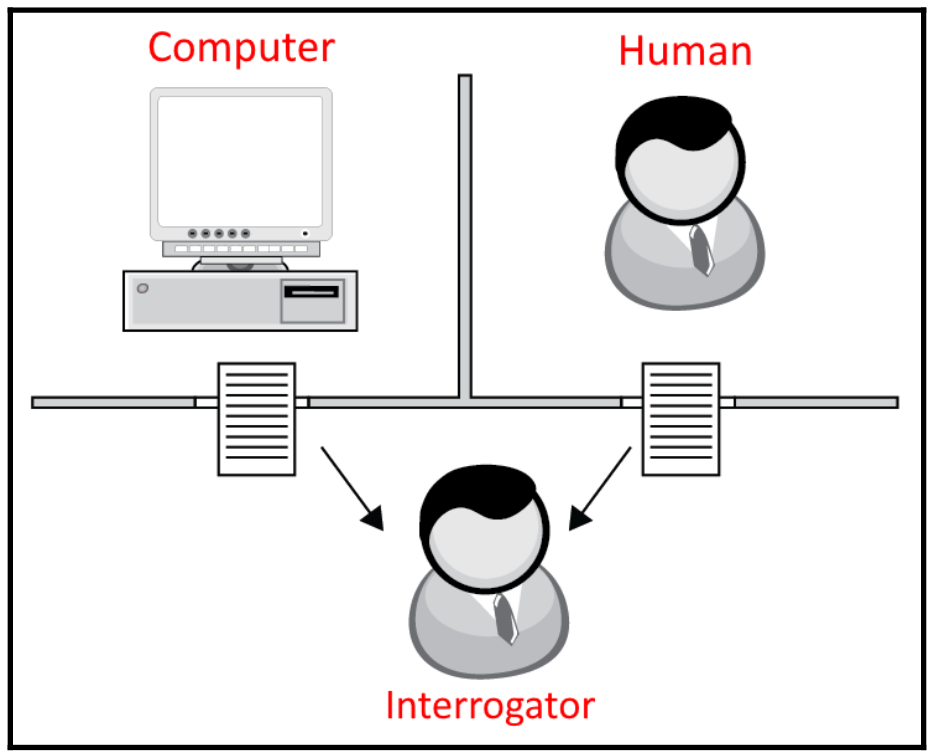
\includegraphics[width=0.6\textwidth]{content/Section-3/Chapter-15/1}
\end{center}

当你开始深入人工智能领域时,智能的定义就变得越来越模糊。可以以任何形式向机器提问:文本、音频、可视形式等。有许多东西可能永远无法在机器中实现,比如:面部表情。有时候人们通过对方的表情来理解对方的心情。你不能确定机器人是否能够理解甚至能够模仿脸上的情绪。没人教过我们在生气的时候要表现出生气的样子,没人教过我们要有情感,它们就在那里。很难说是否有一天,类似的东西是否也会出现在机器上。 \par
说到人工智能,大多数时候我们都认为它是一个说话和行为与人类相似的机器人。但是当你作为一个程序员去分析它的时候,你会遇到很多子领域,每一个都需要花很多时间去理解。许多领域都有很多任务在进行中或处于早期研究阶段。以下是一些你可能会在职业生涯中感兴趣的人工智能子领域: \par

\begin{itemize}
	\item 计算机视觉:设计视觉物体识别的算法,并通过分析物体的视觉表现来理解物体。人类很容易在人群中发现一张熟悉的面孔,但为机器实现类似的功能可能需要花费很多时间来获得与人类相同的精度。
	\item 自然语言处理(NPL):机器对文本的语言分析。在很多领域都有应用,比如机器翻译。想象一下,计算机完全理解人类书写的文本,这样我们就可以告诉它该做什么,而不是花几个月的时间学习编程语言。
	\item 知识推理:这似乎是机器智能行为的目标。知识推理是关于使机器进行推理,并根据它们所拥有的信息提供解决方案,例如:通过检查医疗状况提供诊断。
	\item ML:一个研究算法和统计模型的领域,利用机器在没有明确指令的情况下执行任务。ML算法依赖于模式和推理,而不是直接指令。也就是说,ML允许机器自己完成工作,无需人类参与。
\end{itemize}

\noindent\textbf{}\ \par
\textbf{计算机视觉} \ \par
计算机视觉是一个综合性的研究领域,有很多正在进行的研究项目。它几乎涉及所有与视觉数据处理相关的内容。它在各个领域有着广泛的应用,例如:人脸识别软件处理来自城市各个摄像头的数据,以寻找和确定犯罪嫌疑人,或者光学字符识别软件从包含该数据的图像中生成文本。结合一些增强现实(AR)技术,该软件能够将图像中的文本翻译成用户熟悉的语言。 \par
这一领域的研究正日益取得进展。与人工智能系统相结合,计算机视觉是一个让机器像我们一样感知世界的领域。然而,对我们来说,一个简单的任务,在计算机视觉方面却具有挑战性,例如:当我们在图像中看到一个物体时,我们很容易看出它的尺寸。例如,下面的图片代表了一辆自行车的前视图: \par

\begin{center}
	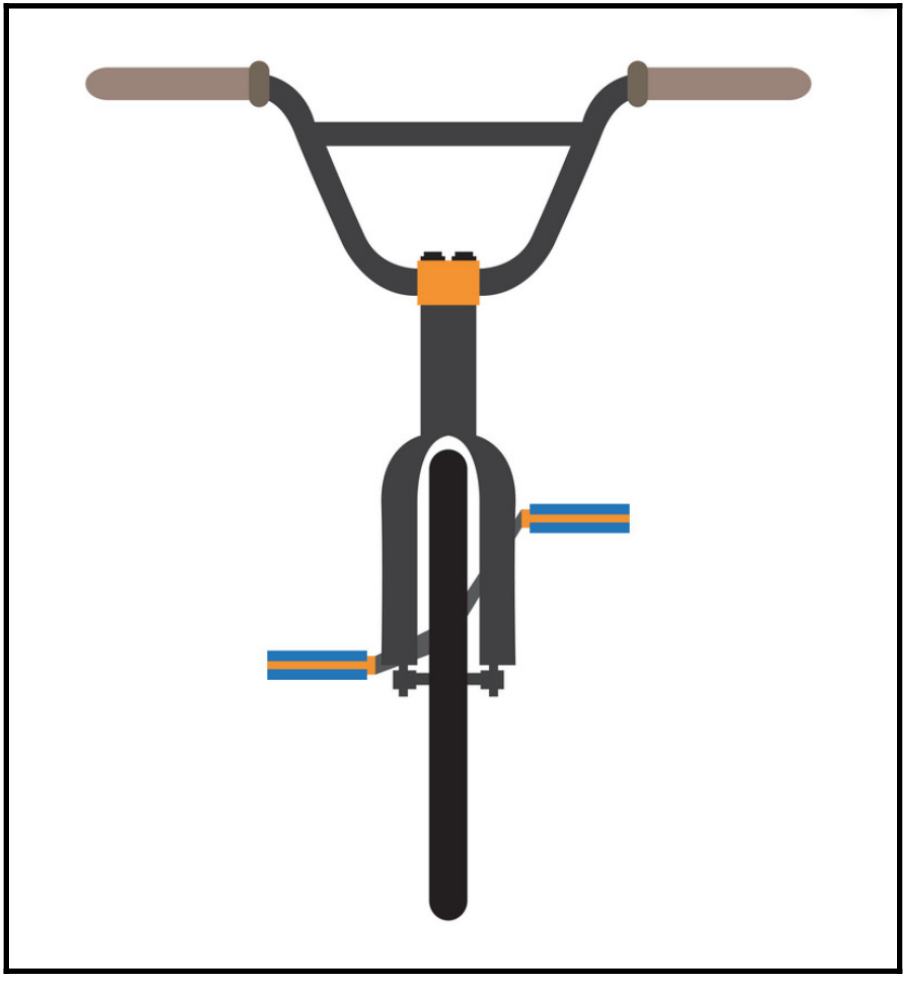
\includegraphics[width=0.6\textwidth]{content/Section-3/Chapter-15/2}
\end{center}

即使我们没有提到这是一辆自行车,人类也不难判断出来。很明显,底部中间的黑线是自行车的前轮。很难让电脑明白这是一个轮子。电脑看到的都是像素的集合,其中一些有相同的颜色: \par

\begin{center}
	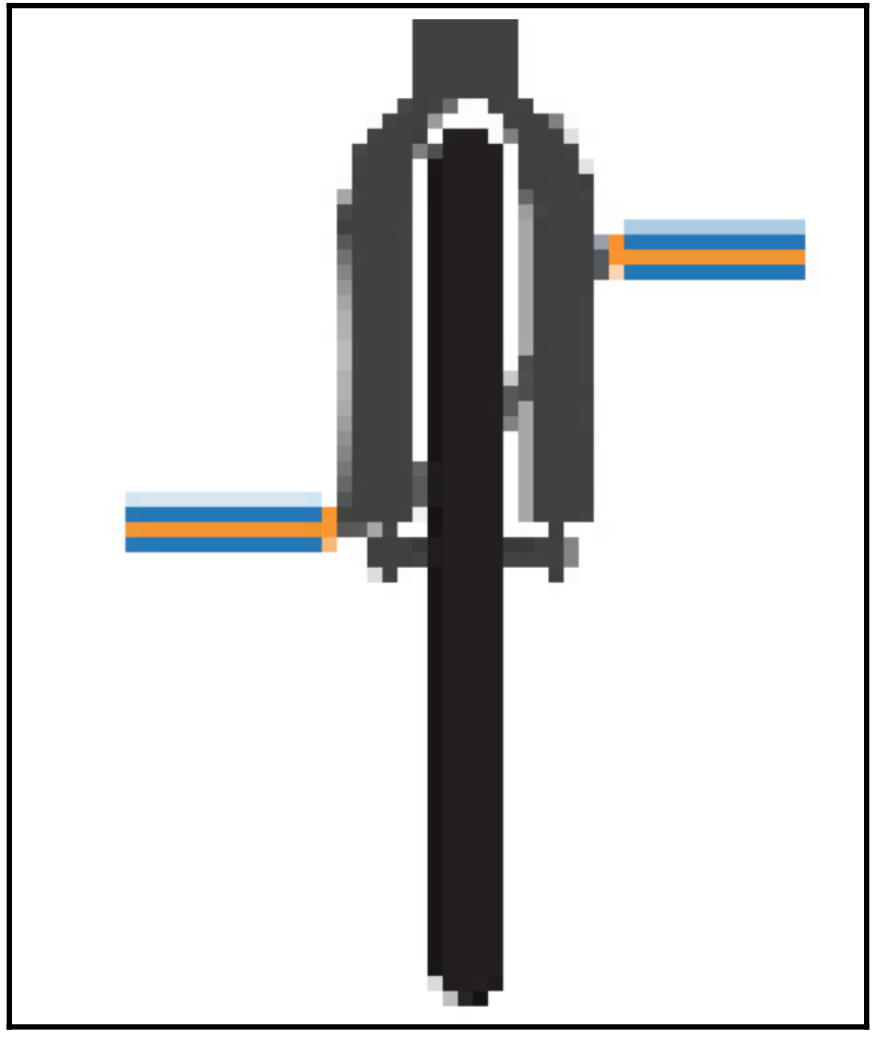
\includegraphics[width=0.6\textwidth]{content/Section-3/Chapter-15/3}
\end{center}

除了理解自行车的车轮之外,还应该推断出这辆自行车一定有另一个在图像中看不到的车轮。同样,我们可能会猜测自行车的大致大小,而计算机从图像中确定它是一个综合性的任务。也就是说,在我们看来,这个简单的事情可能会成为对计算机视觉的真正挑战。 \par

\hspace*{\fill} \\ %插入空行

\includegraphics[width=0.05\textwidth]{images/warn}
我们建议在计算机视觉任务中使用OpenCV库。这是一个用C和C++编写的跨平台库。OpenCV代表了一组针对实时计算机视觉的功能,包括但不限于面部识别、手势识别、运动理解、运动跟踪等特征。 \par
\noindent\textbf{}\ \par

计算机视觉的典型任务包括物体识别、识别和检测。物体识别是理解物体是前一幅图像中的一辆车。识别是对一个对象的单个实例的识别,例如:前面图像中自行车的轮子。目标检测任务可能包括从自行车的图像中发现损坏的区域。所有这些任务与ML算法结合起来,可能组成一个全面的软件,它可以像人类一样了解周围环境。 \par

\noindent\textbf{}\ \par
\textbf{NLP} \ \par
另一个有趣的研究领域是自然语言处理。NLP致力于让计算机理解人类语言,更普遍的方法是自动语音识别和自然语言理解,这是目前虚拟助手的一个关键特性。今天,使用语言控制手机要求它在网络上搜索东西已经不再是魔术了。所有的过程都是由复杂的算法在语音和文本分析。下图显示了会话代理背后发生的流程的高级视图: \par

\begin{center}
	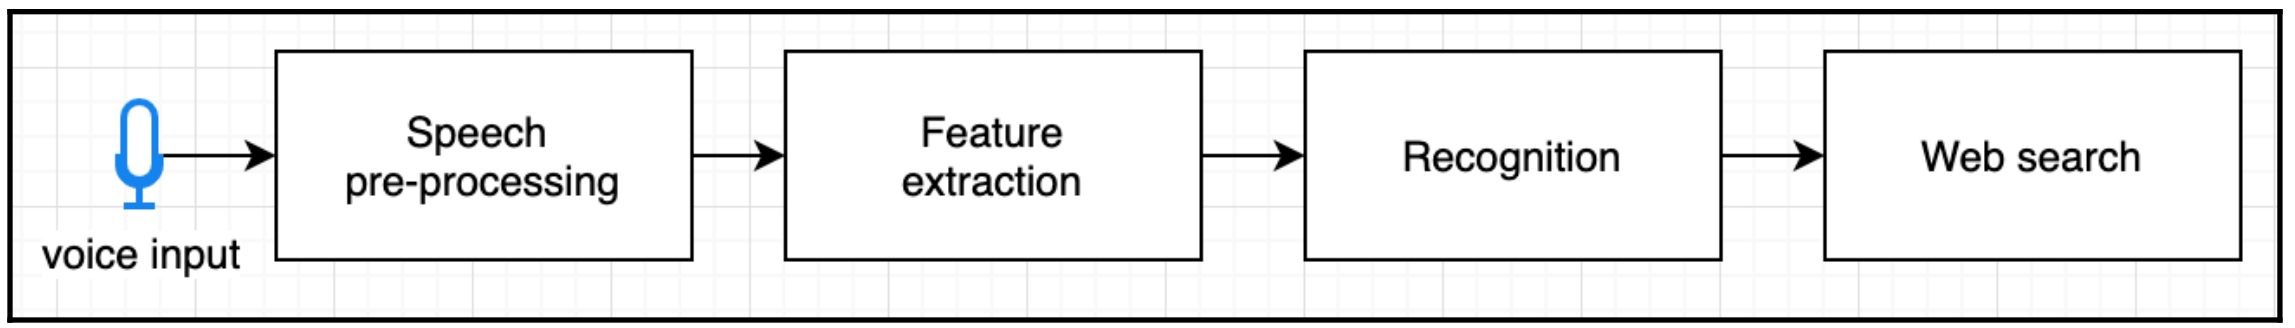
\includegraphics[width=0.6\textwidth]{content/Section-3/Chapter-15/4}
\end{center}

许多语言处理任务都与Web有关。搜索引擎处理用户输入,以便在Web上的数百万文档中进行搜索,这是自然语言处理最热门的应用之一。搜索引擎设计的主要关注点之一是处理文本数据。搜索引擎不能仅仅存储所有的网站并对用户的第一个匹配的查询作出响应。在NLP中有许多具有复杂实现的任务。假设我们正在设计一个程序,它被输入一个文本文档,我们应该输出文档中的句子。识别一个句子的开头和结尾是一项复杂的任务。下面的句子是一个简单的例子: \par

\texttt{I love studying C++. It's hard, but interesting.} \par

程序将输出两个句子: \par

\texttt{I love studying C++.} \par
\texttt{It's hard, but interesting.} \par

就编码任务而言,我们只搜索.(点)字符,并确保第一个单词以大写字母开头。如果一个句子具有以下形式,程序将如何表现? \par

\texttt{I love studying C++!} \par

由于在句子末尾有一个感叹号,我们应该重新访问我们的程序,添加另一个识别句子结尾的规则。如果句子是这样结束的呢? \par

\texttt{It's hard, but interesting...} \par

越来越多的规则和定义引入到具有完整功能的句子提取器中。在解决NLP任务时,利用ML将我们引向一个更明智的方向。 \par
另一个与语言相关的任务是机器翻译,它将文档从一种语言自动翻译成另一种语言。此外,需要注意的是,建立一个全面的NLP系统将有利于其他领域的研究,如知识推理。 \par

\noindent\textbf{}\ \par
\textbf{知识推理} \ \par
知识推理使计算机以与人类相似的方式思考和推理。想象一下和机器对话,开头是这样的: \par
\par
\texttt{[Human] 你好!} \par
\texttt{[Machine] 你好!} \par
\par
我们可以通过编程让机器回答特定的问题或理解用户输入的复杂文本,但要根据以往的经验来判断机器的原因要困难得多。例如,以下推理是这项研究的目标之一: \par
\par
\texttt{[Human] 我昨天走路的时候下着雨。} \par
\texttt{[Machine] 雨中漫步很不错哦。} \par
\texttt{[Human] 下次我应该穿得暖和点。} \par
\texttt{[Machine] 你说的对。} \par
\texttt{[Human] 我好像发烧了。} \par
\textbf{[Machine] 你昨天感冒了吗?} \par
\texttt{[Human] 我想是的。} \par
\par
虽然人类很容易就能发现感冒和下雨之间的联系,但这个程序很难推导出这一点。它一定会把下雨和寒冷联系在一起,把发烧和感冒联系在一起。它还应该记住之前的输入,以便智能地保存。 \par
前面提到的所有研究领域都是开发者可以深入研究的领域。最后,ML通常是所有其他领域的基础,为每个特定的应用设计算法和模型。 \par

\noindent\textbf{}\ \par
\textbf{机器学习} \ \par
ML将我们带到了一个全新的水平,让机器像人类一样执行任务,甚至可能做得更好。与我们前面介绍的领域相比,ML的目标是构建不需要特定指令就能完成任务的系统。在开发人工智能机器的过程中,我们应该仔细看看人类的智能。出生时,孩子不会表现出聪明的行为,但开始慢慢地熟悉周围的世界。没有记录证据表明有任何一个1个月大的孩子解微分方程或作曲。就像孩子学习和发现世界一样,ML关心的是建立直接执行任务的基础模型,而不是能够学习如何去做。这就是让系统执行预先设定好的指令和让它自己去做的根本区别。 \par
当一个孩子开始走路、拿东西、说话、问问题的时候,他们就是在一步步地获得关于世界的知识。她或他拿了一本书,尝了尝它的味道,迟早会停止把书当作可食用的东西来咀嚼。年复一年,孩子打开书页,在书中寻找图像和组成文字的小图形。又过了几年,孩子开始读这些书。多年来,大脑变得越来越复杂,神经元之间产生了越来越多的连接,成为一个有智慧的人。 \par
想象一个系统,它有一些神奇的算法和模型。把一堆数据喂给它,它的理解能力就会越来越强,就像孩子通过视觉(眼睛看)、嗅觉、味道等形式对输入数据进行处理来认识世界一样。后来,通过发展一种提问的方式,孩子能够理解词语,并将这些词语与现实世界中的物体,甚至是无形的概念联系起来。ML系统的作用方式几乎相同。它们对输入数据进行处理,并产生一些符合我们预期结果的输出。下图说明了这个想法: \par

\begin{center}
	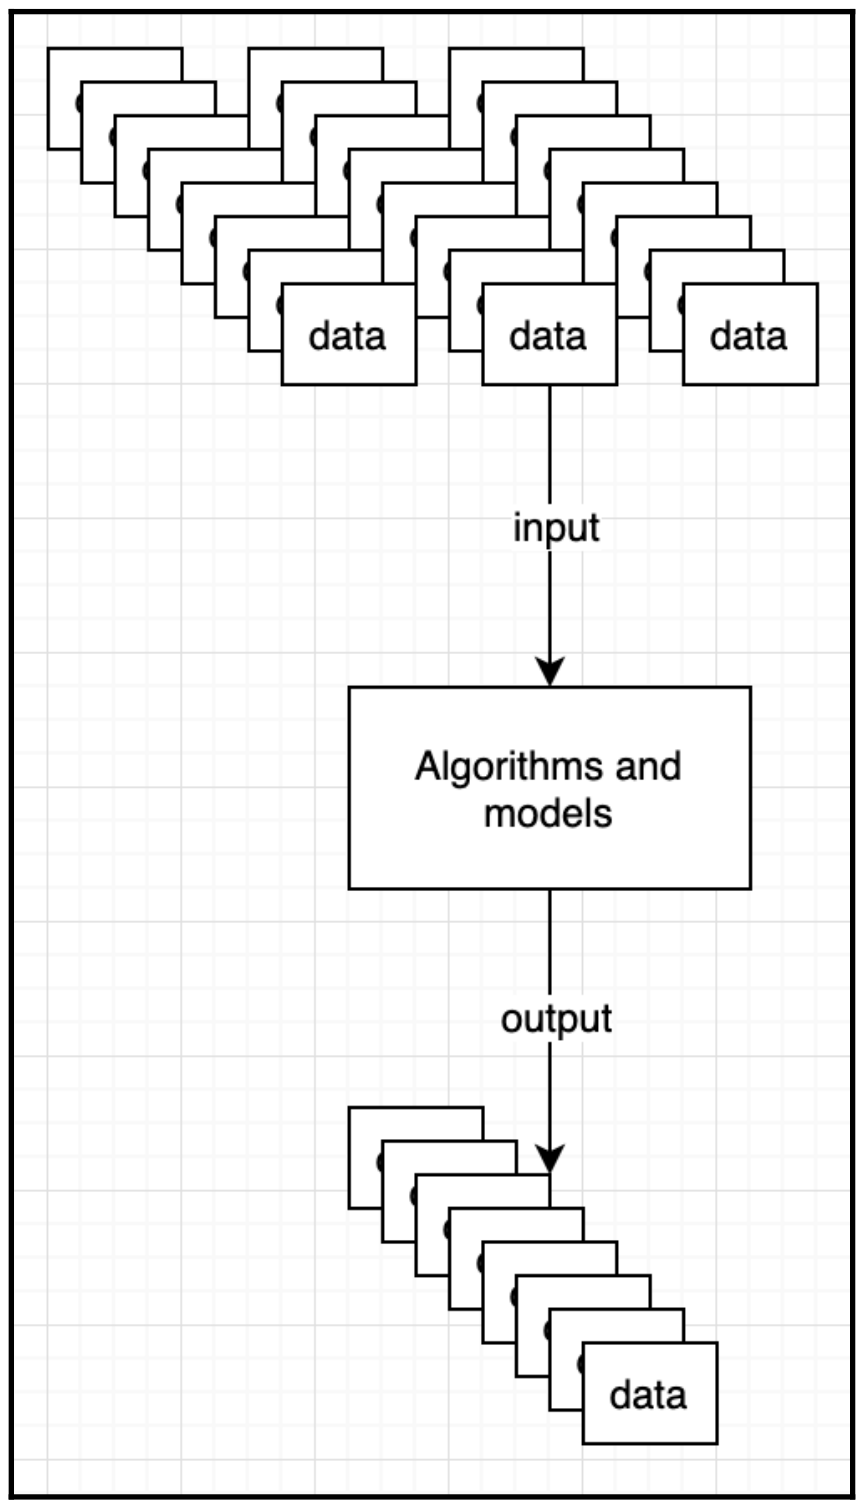
\includegraphics[width=0.6\textwidth]{content/Section-3/Chapter-15/5}
\end{center}

现在让我们更深入地研究ML。和往常一样,理解新事物的最好方法是先尝试实现它。 \par

\noindent\textbf{}\ \par
\textbf{理解机器学习} \ \par
ML是一个大的研究领域,有很多研究正在进行中,并且正在迅速扩展。要了解ML,首先要了解学习的本质。思考和推理是使我们人类与众不同的关键概念。ML的核心是使系统学习和使用知识来执行任务。您可能还记得学习编程的第一步,必须学习新的概念,构建抽象,使大脑理解程序执行背后发生的事情。之后,你应该使用那些小组件构建复杂系统,这些组件包括关键词,指示,条件语句,函数,类等。 \par
然而,ML程序不同于我们通常创建的程序。看看下面的代码: \par

\begin{lstlisting}[caption={}]
int calculate()
{
	int a{14};
	int b{27};
	int c{a + b};
	return c;
}
\end{lstlisting}

简单的先例程序做我们指示它做的事情。它包含了几条简单的指令,指向表示a和b的和的变量c。我们可以修改函数,以接受用户输入如下: \par

\begin{lstlisting}[caption={}]
int calculate(int a, int b)
{
	int c{a + b};
	return c;
}
\end{lstlisting}

前面的函数不会获得任何智能。无论我们调用了多少次calculate()函数都没有关系。输入的数字也无关紧要。该函数表示指令的集合。我们甚至可以说是硬编码指令的集合,函数永远不会修改自己的指令,使其根据输入表现出不同的行为。然而,我们可以引入一些逻辑——让它在每次接收到负数时返回0: \par

\begin{lstlisting}[caption={}]
int calculate(int a, int b)
{
	if (a < 0 && b < 0) {
		return 0;
	}
	int c{a + b};
	return c;
}
\end{lstlisting}

条件语句引入了最简单的决策形式,该函数根据其输入做出决策。我们可以添加越来越多的条件,这样函数就会增长,并有一个复杂的实现。然而,再多的条件语句也不能使它变得聪明,因为这不是代码自己提出的东西。这就是我们在处理程序时所面临的限制。他们会按照我们设定的程序行动。我们决定他们的行为。他们总是服从,只要我们不引入漏洞。 \par
现在,想象一个ML算法在运行。假设calculate()函数具有某种魔力,因此它根据输入返回一个值。假设它有以下形式: \par

\begin{lstlisting}[caption={}]
int calculate(int a, int b)
{
	// some magic
	// return value
}
\end{lstlisting}

现在,假设我们正在调用calculate(),并将2和4作为它的参数传递,希望它将计算它们的和并返回6。另外,想象一下我们可以通过某种方式告诉它结果是否符合我们的预期。一段时间后,函数的行为方式是它理解如何使用这些输入值并返回它们的和。下面我们要构建的类代表了我们理解ML的第一步。 \par

\noindent\textbf{}\ \par
\textbf{设计一个可以学习的算法} \ \par
下面的类代表了一台计算机器。它包含四个算术运算,并期望我们提供如何计算输入值的示例: \par

\begin{lstlisting}[caption={}]
struct Example
{
	int input1;
	int input2;
	int output;
};
class CalculationMachine
{
public:
	using Examples = std::vector<Example>;
	// pass calculation examples through the setExamples()
	void setExamples(const Examples& examples);
	
	// the main function of interest
	// returns the result of the calculation
	int calculate(int a, int b);

private:
	// this function pointer will point to
	// one of the arithmetic functions below
	int (*fptr_)(int, int) = nullptr;
	
private:
	// set of arithmetic functions
	static int sum(int, int);
	static int subtract(int, int);
	static int multiply(int, int);
	static int divide(int, int);
};
\end{lstlisting}

在使用calculate()函数之前,我们应该提供一个setExamples()函数的示例列表。下面是我们提供给CalculationMachine的一个例子: \par

\begin{lstlisting}[caption={}]
3 4 7
2 2 4
5 5 10
4 5 9
\end{lstlisting}

每行中的前两个数字表示输入参数,第三个数字是运算的结果。setExamples()函数是计算机器如何学习使用正确的算术函数。同样的方法,我们可以从前面的例子中猜测发生了什么,同样的方法,CalculationMachine试图找到最适合它的操作。它遍历示例并定义了当调用calculate()时应该使用哪些函数。实现类似如下: \par

\begin{lstlisting}[caption={}]
void CalculationMachine::setExamples(const Examples& examples)
{
	int sum_count{0};
	int sub_count{0};
	int mul_count{0};
	int div_count{0};
	for (const auto& example : Examples) {
		if (CalculationMachine.sum(example.input1, example.input2) ==
		example.output) {
			++sum_count;
		}
		if (CalculationMachine.subtract(example.input1, example.input2) ==
		example.output) {
			++sub_count;
		}
		// the same for multiply() and divide()
	}

	// the function that has the maximum number of correct output results
	// becomes the main function for called by calculate()
	// fptr_ is assigned the winner arithmetic function
}
\end{lstlisting}

从前面的示例中可以看到,该函数调用所有算术函数,并将它们的返回值与示例输出进行比较。每次结果正确时,就会增加特定函数正确答案的数量。最后,将正确答案最多的函数赋值给calculate()函数使用的fptr\underline{ },如下所示: \par

\begin{lstlisting}[caption={}]
int CalculationMachine::calculate(int a, int b)
{
	// fptr_ points to the sum() function
	return fptr_(a, b);
}
\end{lstlisting}

我们设计了一个简单的学习算法。setExamples()函数可以重命名为setDataSet()或trainwithexample()或类似的东西。关于CalculationMachine的例子的要点是,我们定义了一个模型和使用它的算法,我们可以称之为ML。它从数据中学习,能从经验中学习。我们提供给CalculationMachine的例子向量中的每一个记录都可以视为经验,同时计算的性能随经验而提高。也就是说,我们提供的示例越多,它就越有信心选择正确的函数来执行任务。任务是根据两个输入参数计算值。学习的过程本身并不是任务,但学习是完成任务的关键。任务通常被描述为系统应该如何处理一个示例,而示例是功能的集合。尽管在ML术语中,其中每个条目都是另一个特征,矢量数据结构的选择只是一个巧合。ML算法的基本原理之一是对系统进行训练,它可以分为监督算法和无监督算法。让我们了解一下它们的差异,然后再建立ML系统的各种应用。 \par

\noindent\textbf{}\ \par
\textbf{机器学习的类别} \ \par
下面的图表说明了机器学习的分类: \par

\begin{center}
	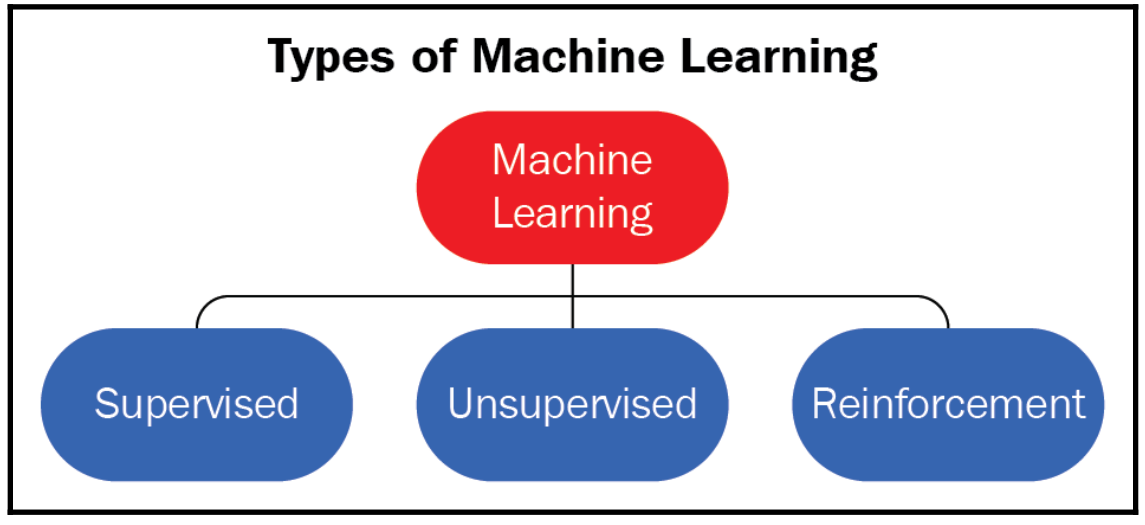
\includegraphics[width=0.8\textwidth]{content/Section-3/Chapter-15/6}
\end{center}

ML算法的分类取决于它们在学习过程中所拥有的经验。我们通常称示例集合为数据集。一些书也使用术语数据点。数据集基本上是表示对目标系统有用的任何数据的集合。可能包括一段时间内的天气测量、某个或多个公司的股票价格列表,或任何其他数据集。虽然数据集可能是未处理的或所谓的原始数据集,但也有针对每个包含的经验的附加信息的数据集。CalculationMachine示例中,我们使用了一个原始数据集,我们已经编程让系统识别出前两个值是操作的操作数,第三个值是操作的结果。如前所述,我们将ML算法分为有监督的和无监督的。 \par
监督学习算法从标记数据集学习,每个记录都包含描述数据的附加信息。calculationmachine是一个监督学习算法的例子。监督学习也称为导师培训。类似讲师使用数据集来教授知识的系统。 \par
有监督的学习算法将能够在学习经验后标记新的未知数据。下面的图表最好地描述了它: \par

\begin{center}
	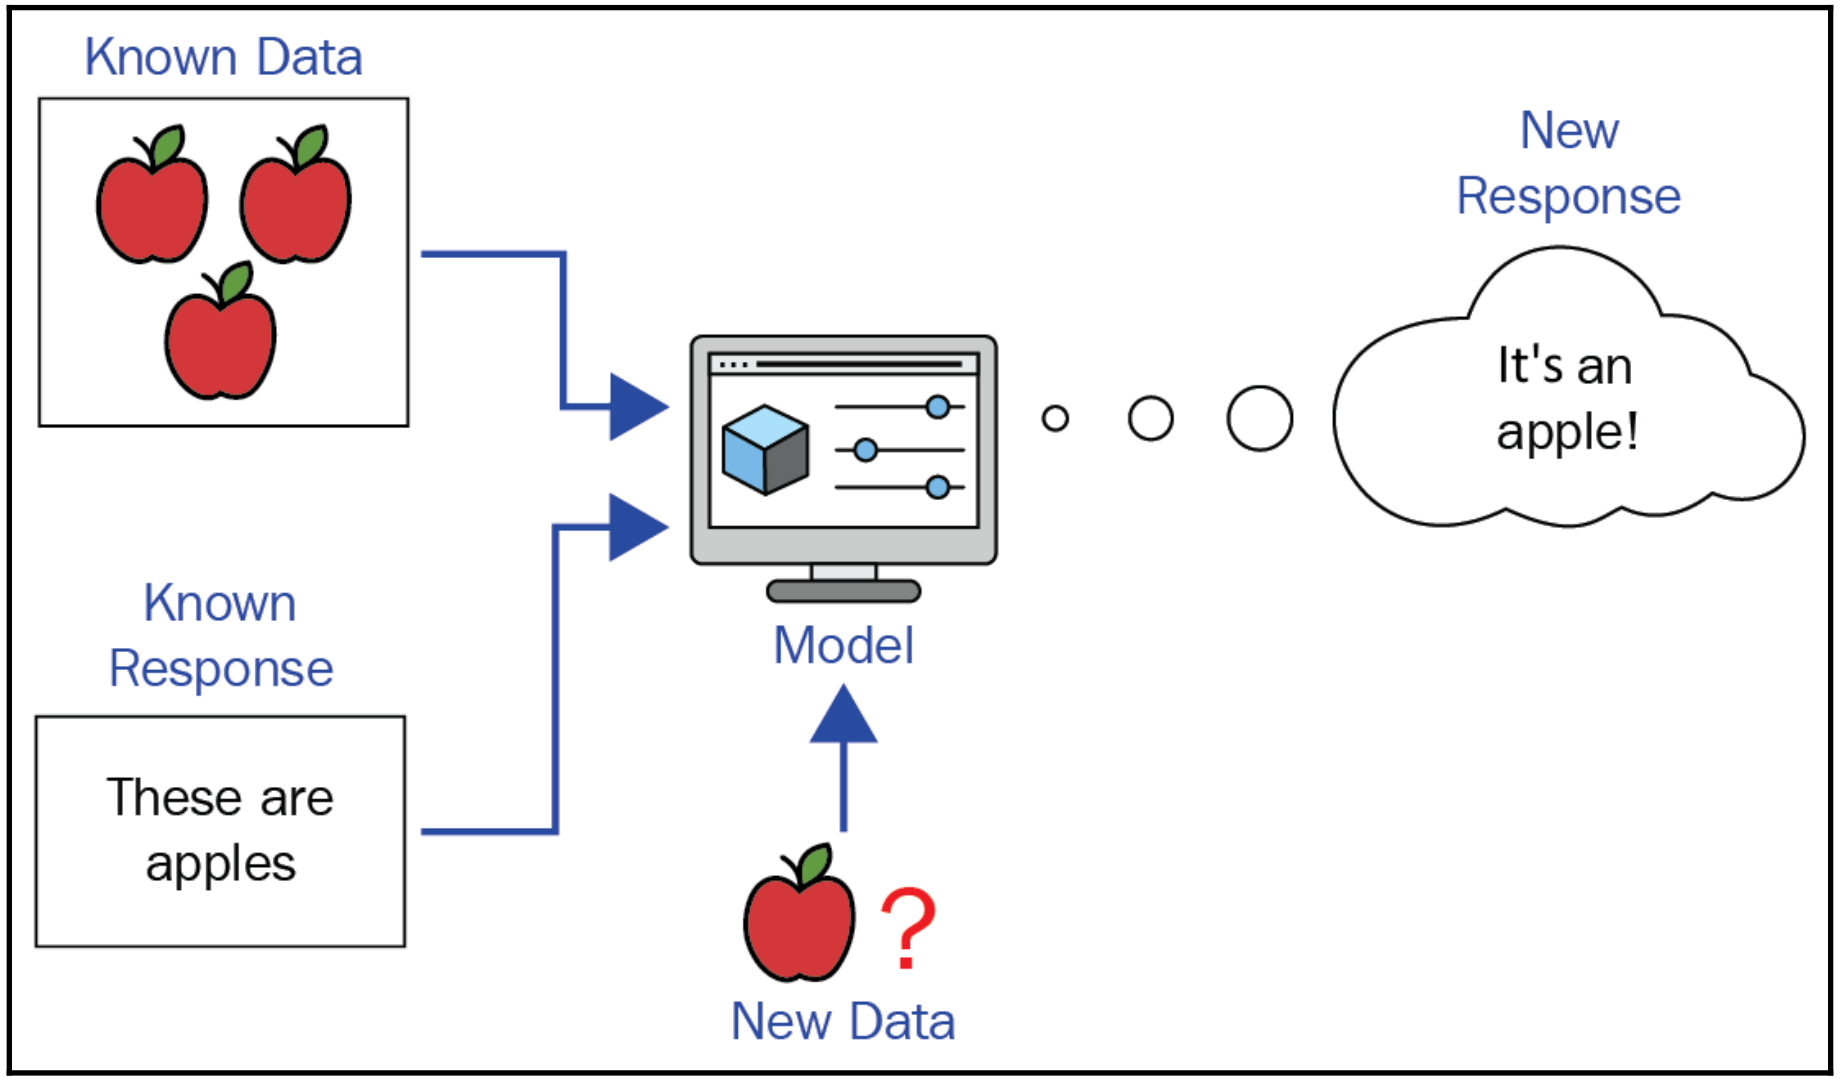
\includegraphics[width=0.8\textwidth]{content/Section-3/Chapter-15/7}
\end{center}

监督学习算法应用的一个很好的例子是电子邮件应用中的垃圾邮件过滤器。用户将电子邮件标记为垃圾邮件或非垃圾邮件,然后系统试图在新收到的电子邮件中发现模式,以检测潜在的垃圾邮件。 \par
CalculationMachine的例子是监督学习的另一个例子。我们提供了以下数据集: \par

\begin{lstlisting}[caption={}]
3 4 7
2 2 4
5 5 10
4 5 9
\end{lstlisting}

我们为CalculationMachine编写了程序,将前两个数字作为输入参数读取,将第三个数字作为应用于输入的函数产生的输出。通过这种方式,我们提供了有关系统应该得到的结果的必要信息。 \par
无监督学习算法甚至更复杂——处理包含一系列特征的数据集,然后找到这些特征的有用属性。无监督学习算法大多是自己定义数据集中的内容。在智能方面,无监督学习方法比监督学习算法更符合智能生物的描述。相比之下,监督学习算法试图预测哪些输入值映射到输出值,而非监督学习算法执行几个操作来发现数据集中的模式。下面的图描述了一种无监督学习算法: \par

\begin{center}
	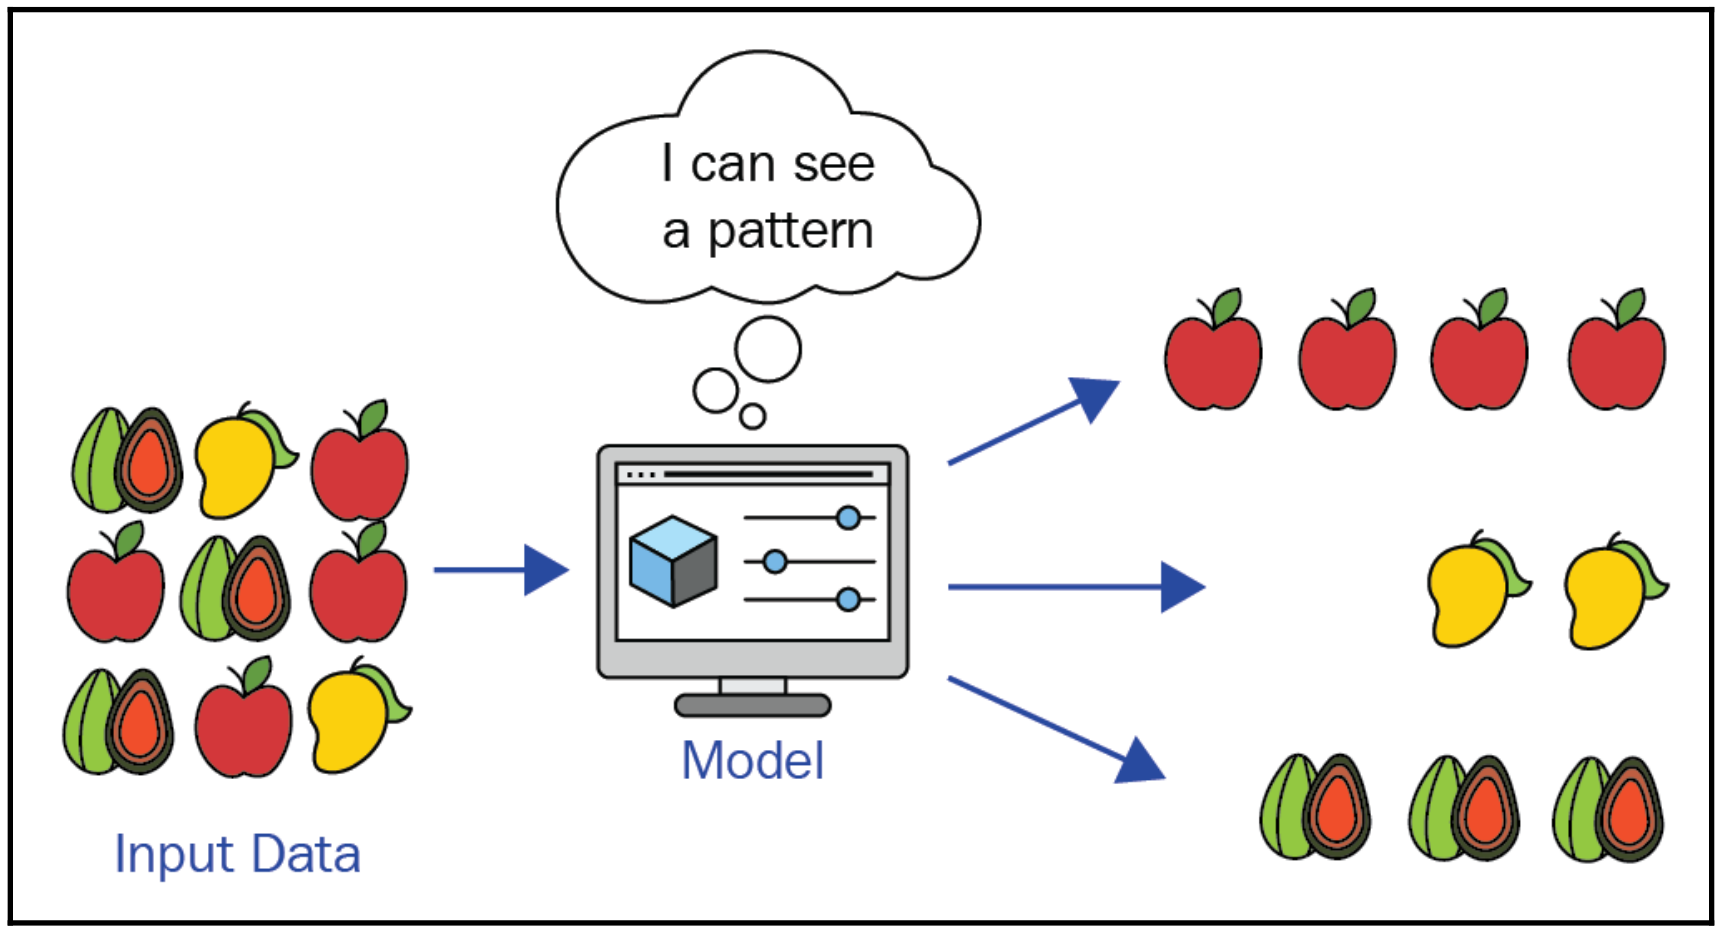
\includegraphics[width=0.8\textwidth]{content/Section-3/Chapter-15/8}
\end{center}

无监督学习算法应用的例子是推荐系统。我们将在下一章中讨论,在那里我们设计了一个网络搜索引擎。推荐系统通过分析用户活动来推荐类似的数据,例如电影推荐。 \par
正如你在前面的例子中看到的,还有强化学习——从错误中学习的算法。在学习系统和经验之间有一个反馈循环,因此强化学习算法与环境相互作用。可能一开始就犯很多错,然后在处理反馈后,进行自我修正以改进算法。学习过程成为任务执行的一部分。想象一下,计算机只接收输入的数字,而不接收计算的结果。对于每一次体验,它将通过应用其中一个算术运算产生一个结果,然后收到反馈。假设它减去这些数字,然后根据反馈进行自我修改,计算出总和。 \par

\noindent\textbf{}\ \par
\textbf{机器学习的应用} \ \par
理解ML的分类有助于更好地将其应用于各种任务。有大量的任务可以用ML解决。我们已经提到分类作为ML算法解决的任务之一。基本上,分类就是对输入进行过滤和排序,以指定输入所属的类别的过程。用ML解决分类问题通常意味着它产生一个将输入映射到特定输出的函数。输出类的概率分布也是一种分类任务。分类任务最好的例子之一是物体识别。输入是一组像素值(换句话说,是一幅图像),输出是标识图像中的对象的值。想象一下,一个机器人可以识别不同种类的工具,并按命令将它们交付给工人,也就是说,一个在车库工作的机械师有一个助手机器人,能够识别螺丝刀并按命令进行工作。 \par
更有挑战性的是在缺少输入的情况下进行分类。前面的例子中,这类似于让机器人来拧紧螺栓。当一些输入缺失时,学习算法必须与多个函数一起操作才能获得成功的结果。例如,机器人助手可能会先拿出钳子,然后再拿出螺丝刀作为正确的解决方案。 \par
与分类类似的是回归,系统被要求预测给定输入的一个数值。不同之处在于输出的格式。回归任务的一个例子是预测股票的未来价格。ML的这些和其他应用使它作为一个研究领域迅速发展。学习算法并不像一开始感觉的那样只是一系列条件语句。它们是基于更全面的构造,模仿人类大脑神经元及其连接。这将引导我们进入下一节,人工神经网络(ANN)的研究。 \par

\noindent\textbf{}\ \par
\textbf{神经网络} \ \par
神经网络是用来识别模式的。它们是模仿人类大脑的,或者说是大脑的神经元和它们的人工对等物——人工神经元。下面的图展示了人脑中的一个神经元: \par

\begin{center}
	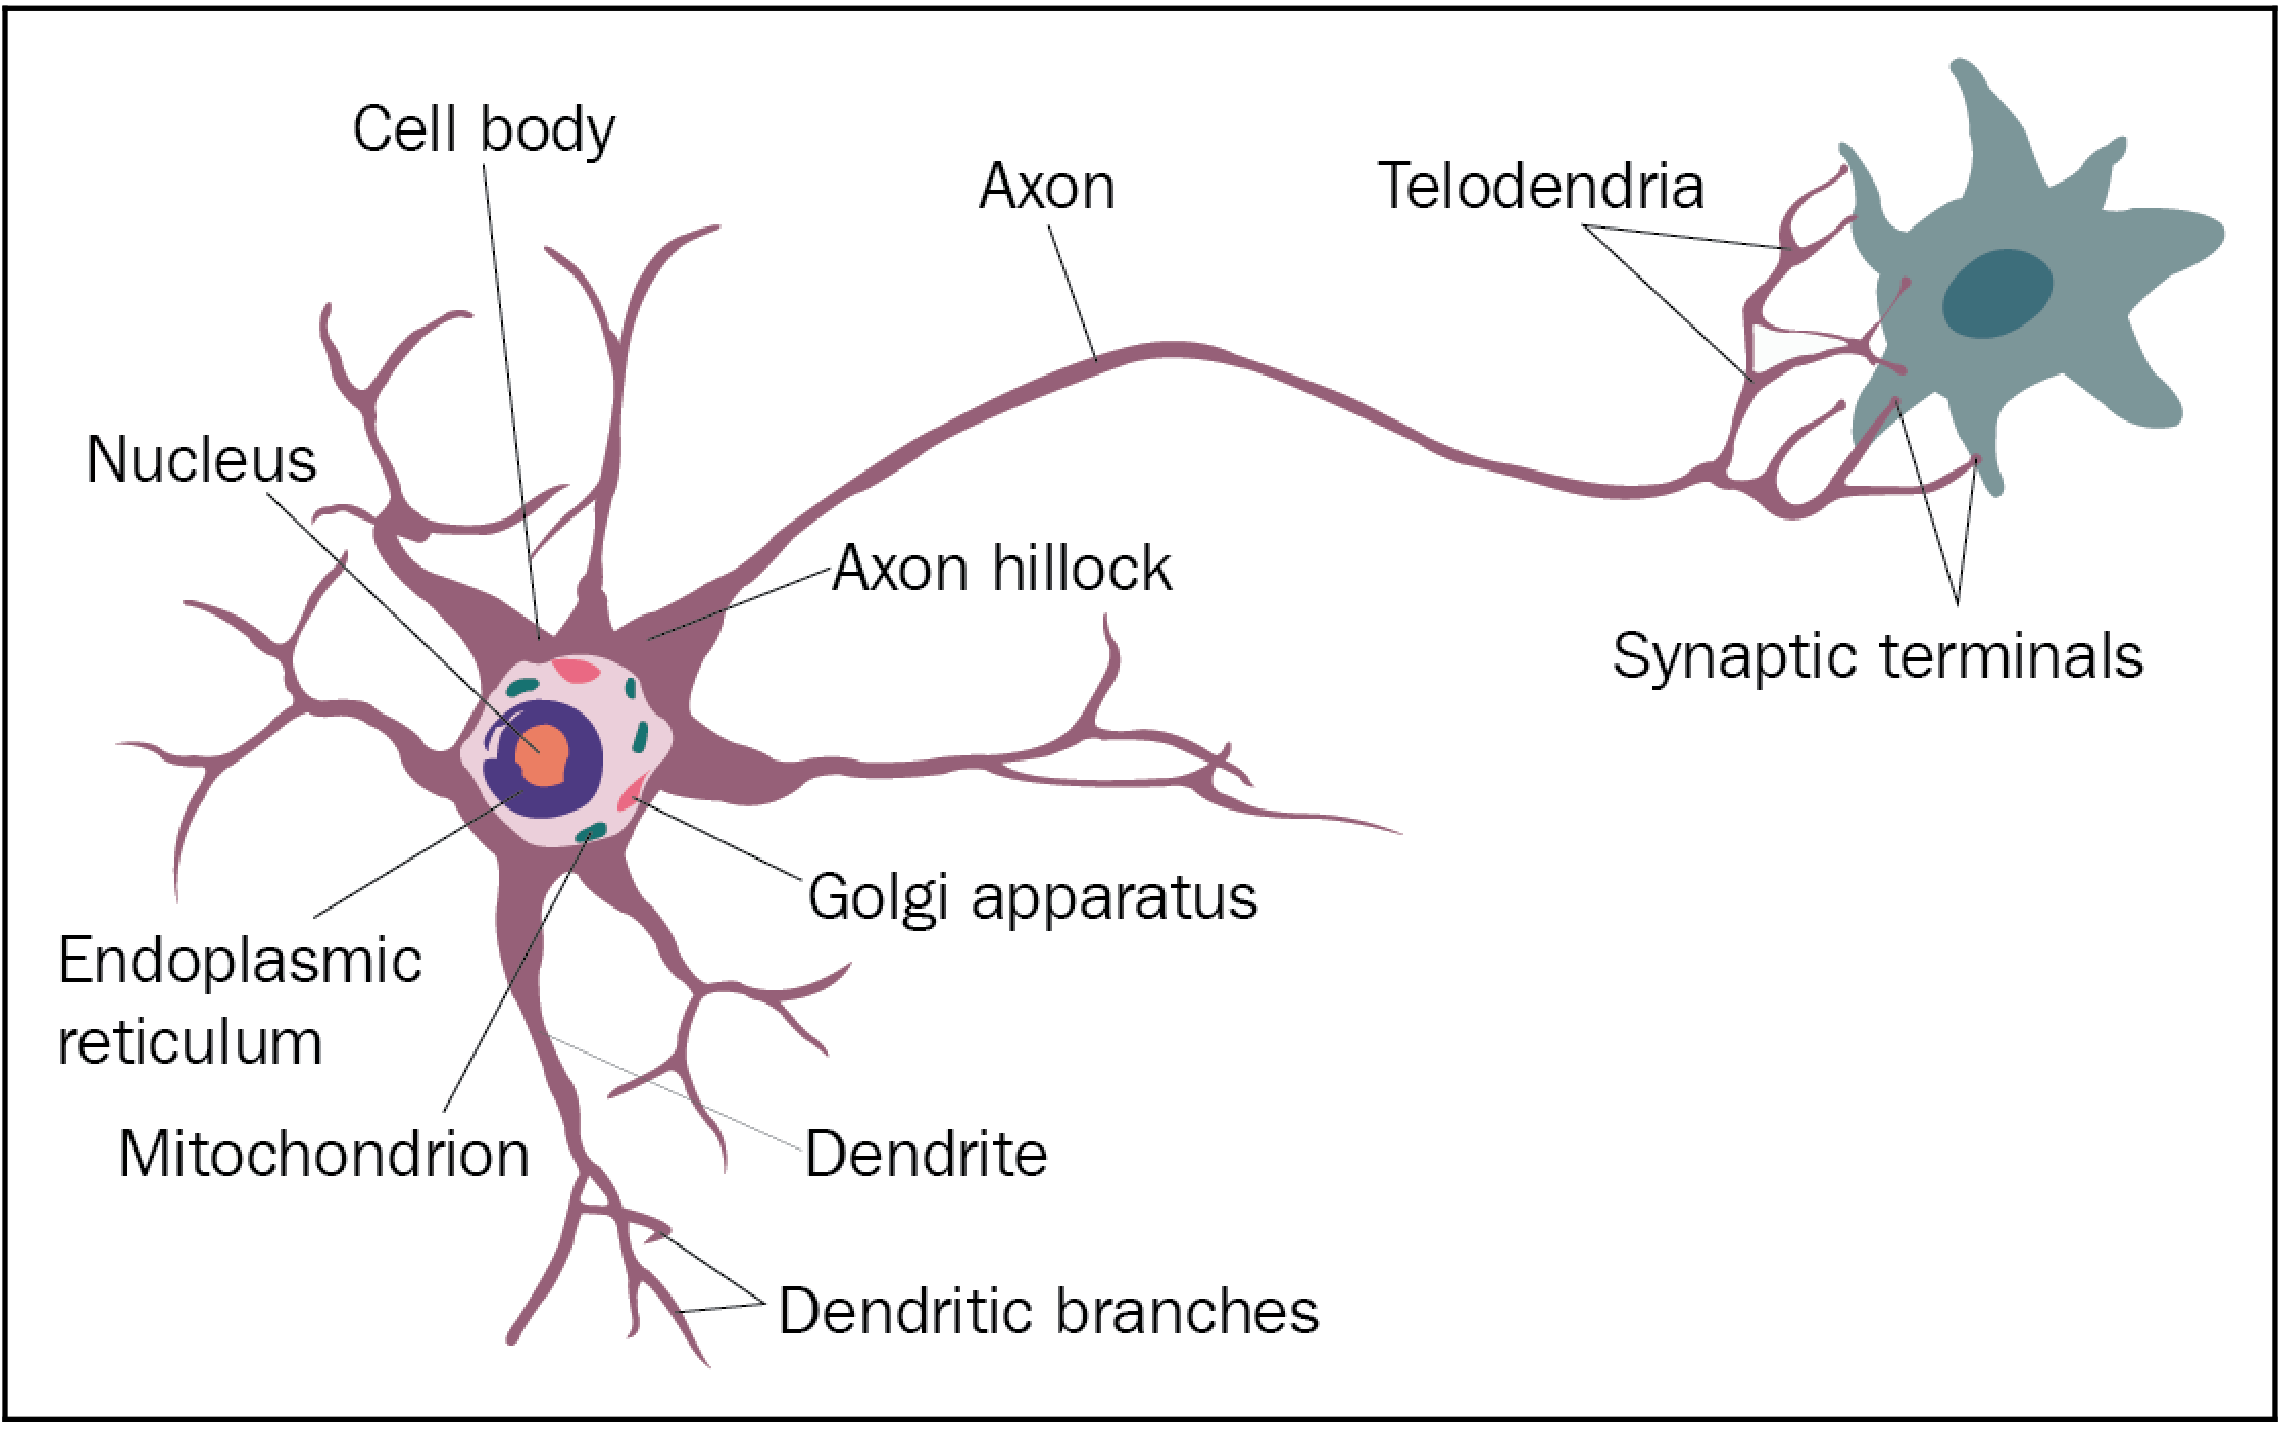
\includegraphics[width=0.8\textwidth]{content/Section-3/Chapter-15/9}
\end{center}

一个神经元通过突触与其他神经元交流。神经元的基本功能是处理一部分数据并根据这些数据产生信号,神经元接受一组输入并产生输出。 \par
下面的图表清楚地说明了为什么人工神经元与人类大脑神经元的结构相似: \par

\begin{center}
	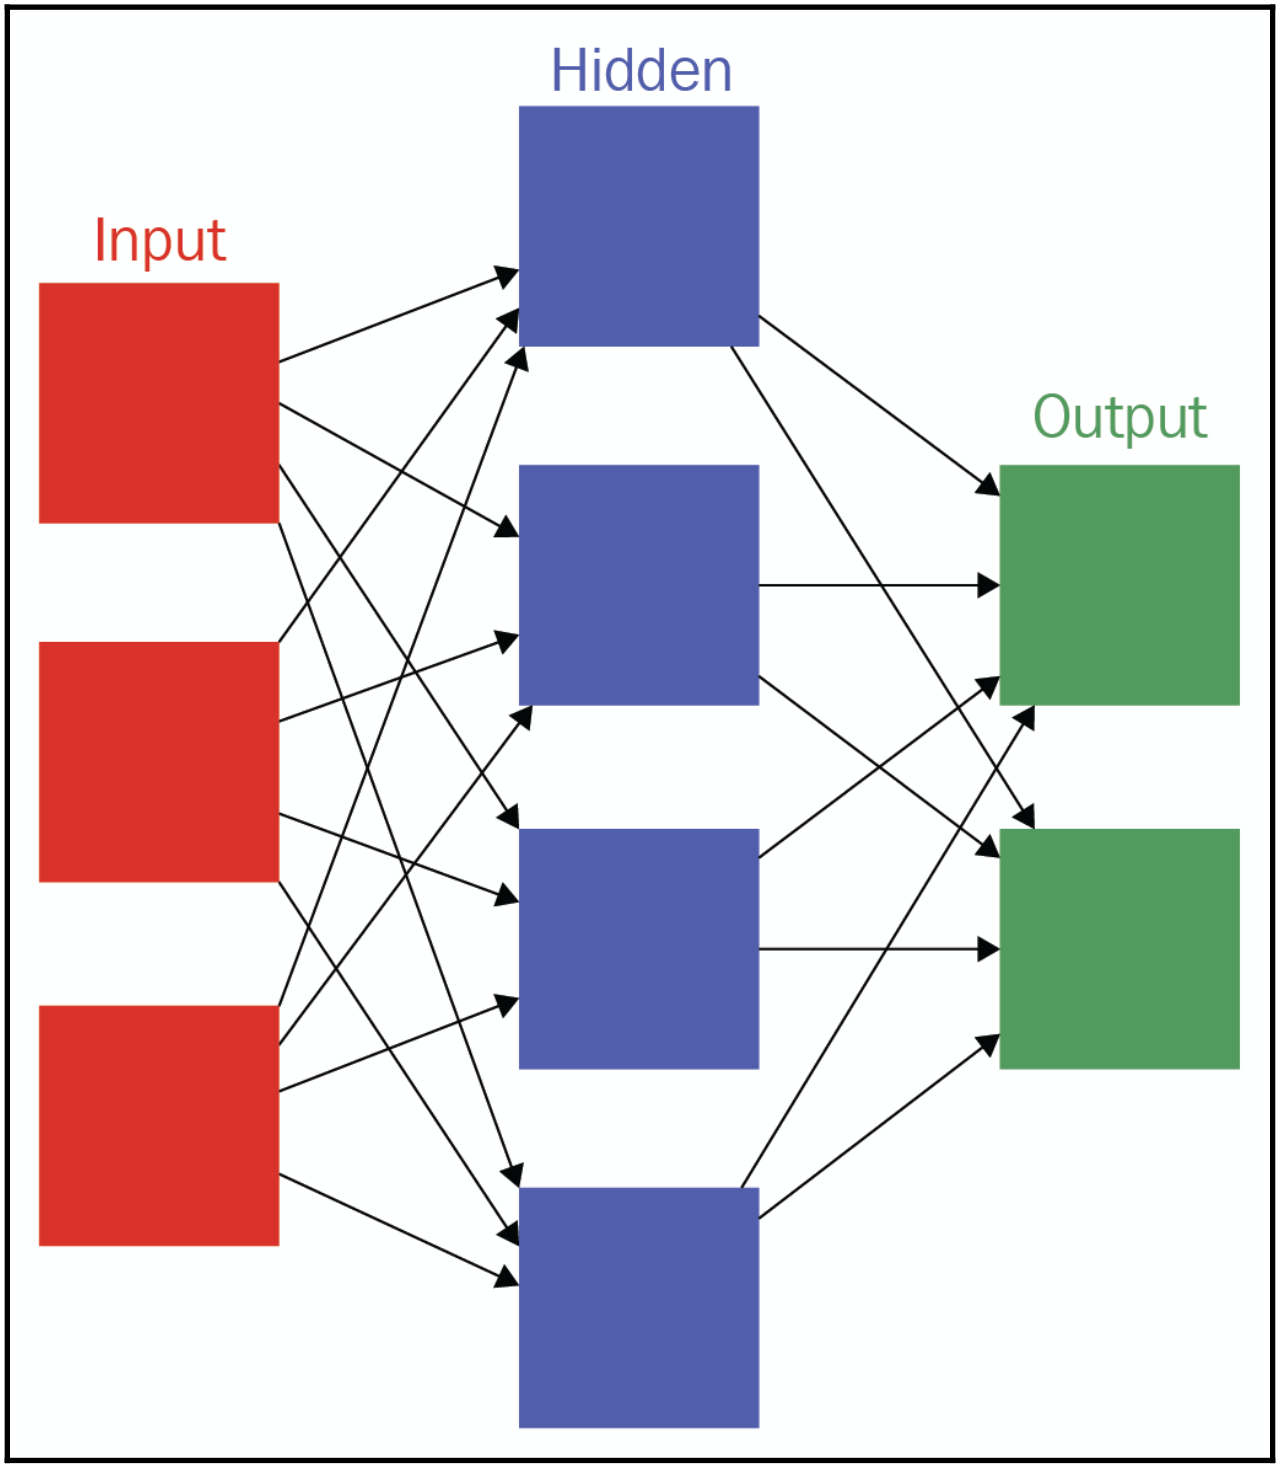
\includegraphics[width=0.5\textwidth]{content/Section-3/Chapter-15/10}
\end{center}

神经网络是自然神经网络的一种简化模型。它代表一组相互连接的节点,每个节点代表一个神经元后的模型。每个节点连接都可以传递类似于生物大脑神经元突触的信号。神经网络是一组有助于聚类和分类的算法。从上图中可以看出,神经网络由三层组成: \par

\begin{itemize}
	\item 输入层
	\item 隐藏层
	\item 输出层
\end{itemize}

输入层表示问题的初始输入数据,例如:图像、音频或文本文件。输出层是完成任务的结果,例如:对文本内容或图像中已识别的对象进行分类。隐藏层使网络产生合理的结果。输入到输出的转换要经过隐藏层,该层要进行大量的分析、处理和修改,以产生输出。 \par
考虑上面的图表,表明神经元可以有多个输入和输出连接。通常,每个连接都有一个权重来指定连接的重要性。上图中的神经元层告诉我们,每一层的神经元都与前一层和后一层的神经元相连。应该注意,在输入层和输出层之间可能有几个隐藏层。输入输出层的主要目的是读取外部数据并返回计算(或推导)的输出,而隐含层的目的是通过学习来适应。学习还包括调整连接和权重,以提高输出精度(这就是ML发挥作用的地方)。所以,如果我们创建一个包含几个隐藏层的复杂神经网络,准备学习和改进,我们就得到了一个人工智能系统。例如,我们来看一下聚类问题,然后再转向回归分析。 \par

\noindent\textbf{}\ \par
\textbf{聚类} \ \par
聚类是指对一组对象进行分组,将它们分布在类似对象的分组中,也称为聚类分析。它是一组技术和算法,目的是将相似的对象分组在一起,产生聚类。最简单的说就是将一组有颜色的物体分成由相同颜色的物体组成的不同组,如下所示: \par

\begin{center}
	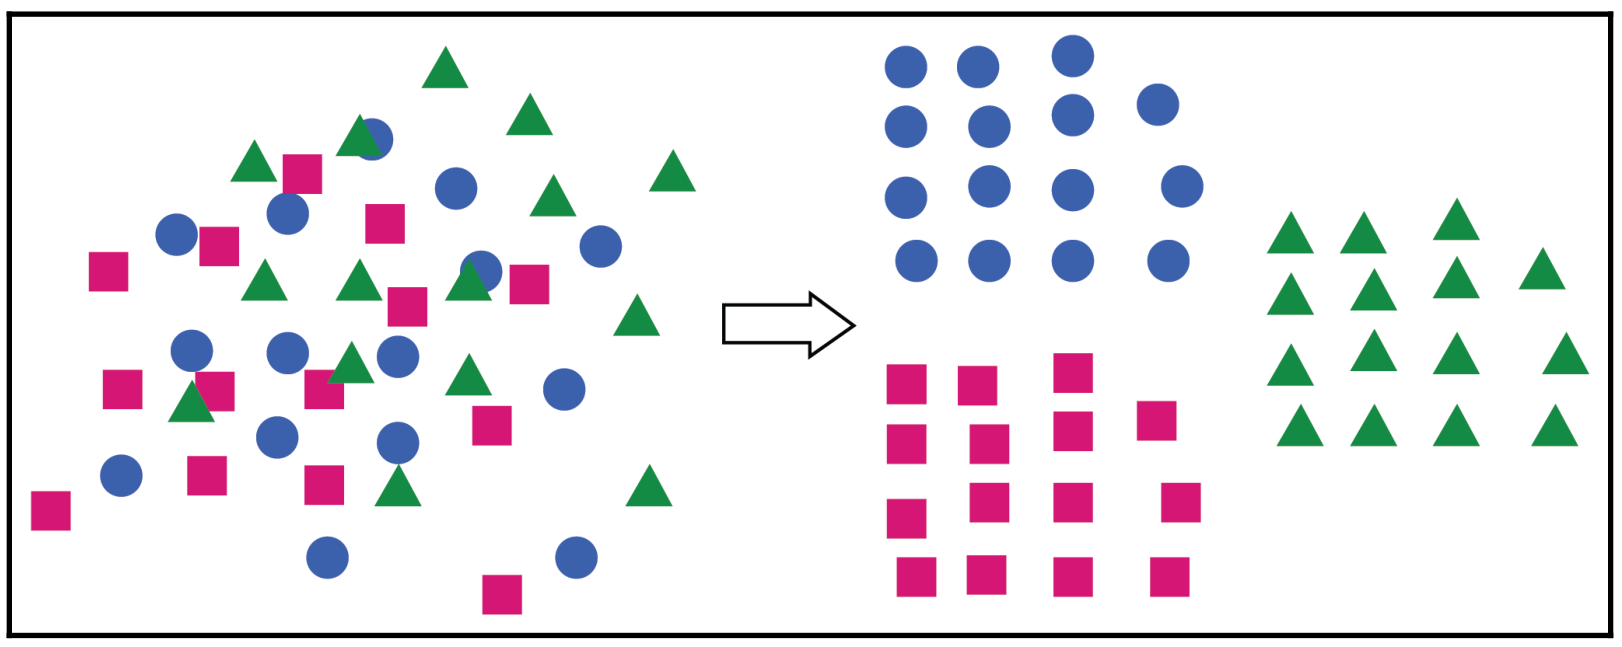
\includegraphics[width=0.8\textwidth]{content/Section-3/Chapter-15/11}
\end{center}

虽然本章中讨论的是人工智能任务,但我们建议你先尝试用目前拥有的知识库来解决问题,让想想我们自己如何通过相似性来给物体分类。首先,我们应该有一个物体的基本概念。在前面的例子中,对象的形状、颜色、尺寸(2D对象的宽度和高度)等。不需要深入了解,一个基本的对象表示可能是这样的: \par

\begin{lstlisting}[caption={}]
struct Object
{
	int color;
	int shape;
	int width;
	int height;
};
\end{lstlisting}

我们考虑这样一个情况,即颜色和形状的值在一定范围内是已定义的。我们可以使用枚举来提高可读性。聚类分析包括对对象进行分析,并对其进行分类。首先想到的是拥有一个接受对象列表的函数。让我们来定义一个: \par

\begin{lstlisting}[caption={}]
using objects_list = std::vector<Object>;
using categorized_table = std::unordered_map<int, objects_list>;
categorized_table clusterize(const objects_list& objects)
{
	// categorization logic
}
\end{lstlisting}

考虑一下实现细节。需要定义聚类点,有可能是颜色,也可能是形状的类型。挑战性在于,它可能是未知的。也就是说,为了防止万一,我们将每个属性的对象分类如下: \par

\begin{lstlisting}[caption={}]
categorized_table clusterize(const objects_list& objects)
{
	categorized_table result;
	for (const auto& obj : objects) {
		result[obj.color].push_back(obj);
		result[obj.shape].push_back(obj);
	}
	return result;
}
\end{lstlisting}

具有相似颜色或形状的对象分组在一个散列表中。虽然前面的代码相当简单,但它承载了根据某种相似标准,对对象进行分组的基本思想。我们在上一个示例中所做的可以描述为硬集群。一个对象要么属于一个集群,要么不属于。相反,软聚类(也称为模糊聚类)可以在一定程度上描述对象所属的聚类。 \par
例如,shape属性的对象相似性可以通过应用于对象的函数的结果来定义。也就是说,如果对象A的形状是正方形,而对象B的形状是菱形,那么该函数定义对象A和对象B是否具有相似的形状。这意味着我们应该更新前面示例中的逻辑,将对象与多个值进行比较,并将它们的形状定义为一个组。通过进一步发展这一思想,我们会得到不同的聚类策略和算法,例如K-means聚类。 \par

\noindent\textbf{}\ \par
\textbf{回归分析} \ \par
回归分析关心的是找出一个值与另一个值的偏差。最简单的理解回归分析的方法是通过数学中的函数图。你可能还记得函数$ f(x) = y $的图像: \par

\begin{center}
	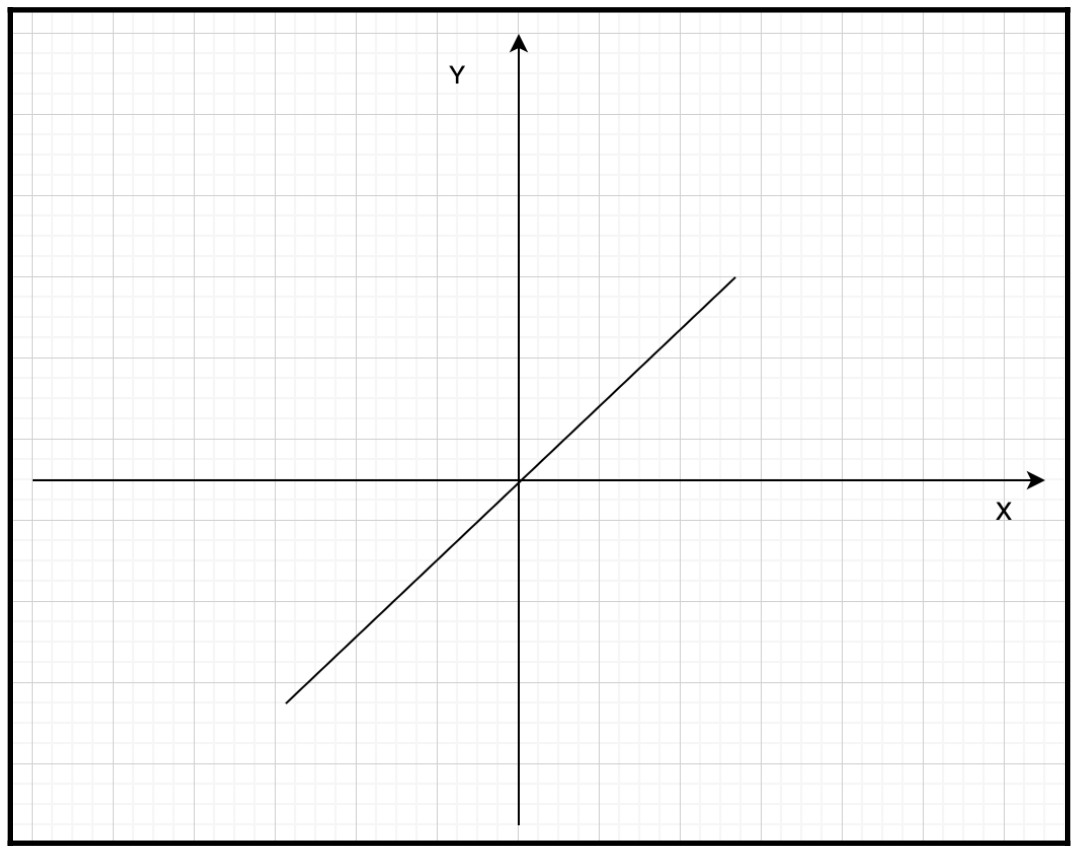
\includegraphics[width=0.8\textwidth]{content/Section-3/Chapter-15/12}
\end{center}

对于每一个x的值,函数的结果是y的一个固定值。回归分析有点类似于前面的图表,因为它关注的是找出变量之间的关系。更具体地说,它估计一个因变量和几个自变量之间的关系。因变量也称为结果,自变量也称为特征。功能的数量可能是一个。 \par
最常见的回归分析形式是线性回归。它看起来与前面的图表相似。下面的例子代表了花费在测试程序上的时间和在发布版本中发现的bug数量之间的关系: \par

\begin{center}
	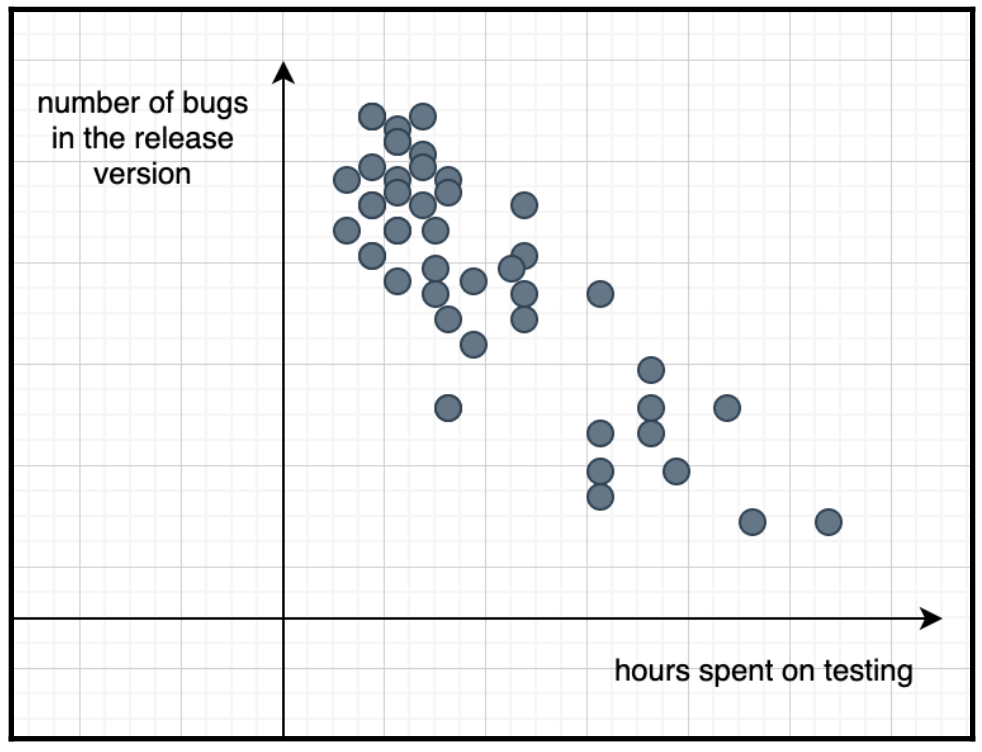
\includegraphics[width=0.8\textwidth]{content/Section-3/Chapter-15/13}
\end{center}

有两种类型的回归:负回归是如上图所示的,随着自变量的减少而因变量的增加。另一方面,正回归对自变量的值递增。 \par
ML中的回归分析是一种预测方法。可以开发一个程序,根据因变量的值来预测结果。ML是一个大领域,涉及的主题非常广泛。尽管开发者倾向于尽可能少地使用数学,但在ML领域是不行的。你仍然需要掌握一些数学科目,以充分利用ML。回归分析强烈依赖于统计学。 \par

\noindent\textbf{}\ \par
\textbf{C++和机器学习} \ \par
ML更多的是关于数学而不是编程,这已经不再是一个秘密了。计算机科学起源于数学,在早期,计算机科学家首先是数学家。你可能熟悉几个著名的科学家,包括艾伦·图灵,约翰·冯·诺伊曼,克劳德·香农,诺伯特·维纳,尼克劳斯·沃斯,唐纳德·克努特还有很多人。他们都是数学家,对技术有着特殊的热爱。在计算机的发展过程中,编程成为了一个对新来者更友好的领域。过去的二三十年里,计算机开发者在开发有用的程序之前不再被迫要学习数学。语言发展成为越来越多的高级工具,几乎每个人都可以编写代码。 \par
有很多框架可以让程序员的工作变得更容易。现在,掌握一些框架或高级编程语言并创建一个新程序需要几周的时间。然而,程序往往会重复。现在构建东西并不难,因为有很多模式和最佳实践在这一过程中帮助我们。数学的作用已经不再是必须,越来越多的人成为程序员,甚至不需要使用数学。这其实不是问题,这更像是技术发展的自然过程。最终,科技的目的是让人类生活得更舒适,工程师也是如此。虽然在20世纪60年代,NASA的工程师们使用计算机进行计算,但那不是我们今天所知道的“计算机”。他们都是真实存在的人,他们有一种特殊的能力叫做计算机,“计算机”意味着他们在数学和解方程方面要比其他人快得多。 \par
现在我们是计算机科学新时代的一部分,数学又回来了。ML工程师现在使用数学的方式,就像数学家在70年代或80年代使用编程语言一样。现在,仅仅了解一种编程语言或框架来设计新的算法或将ML合并到应用程序中是不够的。你也应该至少在一些数学的子领域,如线性代数,统计和概率论。 \par
几乎同样的逻辑也适用于C++。现代语言提供了广泛的开箱即用的功能,而C++开发人员仍在努力设计具有手动内存管理的完美程序。如果你对ML领域做一些快速研究,你会发现大多数库或示例都在使用Python。首先,这可能被视为ML任务中使用的默认语言。然而,ML的工程师们开始触及进化的一个新门槛——性能。这并不新鲜,许多工具仍然在性能敏感的部分使用C++。游戏开发、操作系统、关键任务系统和许多其他基本领域都使用C++(和C)作为标准。现在是C++征服新领域的时候了。我们给读者的最好建议是同时学习ML和C++,因为对于ML工程师来说,可以结合C++以获得最好的性能在实际应用中变得越来越关键。 \par

\noindent\textbf{}\ \par
\textbf{总结} \ \par
介绍了ML的分类和应用。它是一个快速发展的研究领域,在构建智能系统方面有着众多的应用。我们将ML分为有监督、无监督和强化学习算法。每个类别都有自己的应用,如:分类,聚类,回归,和机器翻译。 \par
我们实现了一个简单的学习算法,它基于作为输入的经验定义了一个计算函数。我们称它为用来训练系统的数据集。使用数据集(称为经验)训练是ML系统的关键属性之一。 \par
最后,我们介绍并讨论了人工神经网络在模式识别中的应用。ML和神经网络在解决问题时是密切相关的。本章为您提供了该领域的必要介绍,以及几个任务示例,以便您可以花一些时间深入该主题。这将帮助您了解AI和ML的一般概念,因为在现实世界的应用程序开发中,工程师越来越需要AI和ML。在下一章,我们将学习如何实现一个基于对话框的搜索引擎。 \par

\noindent\textbf{}\ \par
\textbf{问题} \ \par
\begin{enumerate}
	\item ML是什么?
	\item 有监督和无监督学习算法之间有什么区别?
	\item 给出一些ML应用的例子。
	\item 在用一组不同的经验训练CalculationMachine类后,您将如何修改它来改变它的行为?
	\item 神经网络的目的是什么?
\end{enumerate}

\noindent\textbf{}\ \par
\textbf{扩展阅读} \ \par
\begin{itemize}
	\item Artificial Intelligence and Machine Learning Fundamentals, at  https:/​/​www.packtpub.​com/​big-​data-​and-​business-​intelligence/​artificial-intelligence-​and-​machine-​learning-​fundamentals
	\item Machine Learning Fundamentals, at  https:/​/​www.​packtpub.​com/​big-​data-​and-business-​intelligence/​machine-​learning-​fundamentals
	\item Hands-On Machine Learning for Algorithmic Trading, at  https:/​/​www.​packtpub.com/​big-​data-​and-​business-​intelligence/​hands-​machine-​learning-algorithmic-​trading
\end{itemize}

\newpage














